\documentclass[aspectratio=169]{beamer}
\usetheme{default}
\usepackage[absolute,overlay]{textpos}
\usepackage{amsmath}
\usepackage{booktabs}
\usepackage{graphicx}
\usepackage{tabularx}
\usepackage{xcolor}
\usepackage{tikz}
\usetikzlibrary{arrows.meta,backgrounds,calc,decorations.pathreplacing,fit,positioning,shapes.geometric}
\definecolor{NovaNavy}{HTML}{123047}
\definecolor{NovaGrowth}{HTML}{18A67A}
\definecolor{NovaSky}{HTML}{4A90E2}
\definecolor{NovaYellow}{HTML}{F4C95D}
\definecolor{NovaCoral}{HTML}{EF6F61}
\definecolor{NovaPaper}{HTML}{F8FAF7}
\definecolor{NovaInk}{HTML}{20323F}
\colorlet{NovaBlue}{NovaSky}
\colorlet{NovaMint}{NovaGrowth}
\definecolor{SubjectAccent}{HTML}{4A90E2}
\usefonttheme{professionalfonts}
\renewcommand{\familydefault}{\sfdefault}
\setbeamercolor{background canvas}{bg=NovaPaper}
\setbeamercolor{normal text}{fg=NovaInk,bg=NovaPaper}
\setbeamercolor{structure}{fg=NovaBlue}
\setbeamercolor{frametitle}{fg=white,bg=NovaNavy}
\setbeamercolor{title}{fg=white,bg=NovaNavy}
\setbeamercolor{block title}{fg=white,bg=SubjectAccent}
\setbeamercolor{block body}{fg=NovaInk,bg=SubjectAccent!7}
\setbeamercolor{block title alerted}{fg=white,bg=NovaCoral}
\setbeamercolor{block body alerted}{fg=NovaInk,bg=NovaCoral!8}
\setbeamertemplate{blocks}[rounded][shadow=false]
\setbeamerfont{frametitle}{size=\Large,series=\bfseries}
\setbeamerfont{block title}{size=\normalsize,series=\bfseries}
\setbeamertemplate{navigation symbols}{}
\setbeamertemplate{frametitle}{
  \nointerlineskip
  \begin{beamercolorbox}[wd=\paperwidth,ht=0.88cm,dp=0.22cm,leftskip=0.45cm,rightskip=0.45cm]{frametitle}
    \usebeamerfont{frametitle}\insertframetitle\hfill{\small $\Sigma$\hspace{0.2cm}Solve}
  \end{beamercolorbox}
}
\setbeamertemplate{footline}{
  \leavevmode
  \hbox{
    \begin{beamercolorbox}[wd=.82\paperwidth,ht=0.24cm,dp=0.14cm,leftskip=0.45cm]{author in head/foot}
      \scriptsize\color{NovaInk!65}NovaSprout Learning
    \end{beamercolorbox}
    \begin{beamercolorbox}[wd=.18\paperwidth,ht=0.24cm,dp=0.14cm,rightskip=0.45cm plus1fil]{date in head/foot}
      \hfill\scriptsize\color{NovaInk!65}\insertframenumber
    \end{beamercolorbox}
  }
}
\newcommand{\NovaQuestion}[1]{\begin{block}{Think about it}#1\end{block}}
\newcommand{\NovaMisconception}[1]{\begin{alertblock}{Check the model}#1\end{alertblock}}
\title{Sampling Distributions And Standard Error}
\subtitle{Grade 11 Mathematics Sampling distributions, standard error, z-scores, and confidence intervals}
\author{NovaSprout Learning}
\date{}

\begin{document}
\begin{frame}{Learn Sampling distributions, standard error, z-sco...}
\begin{columns}[T]
\begin{column}{0.53\textwidth}
\begin{alertblock}{Key idea}
\small For a Grade 11 learner beginning statistical inference.
\end{alertblock}

\begin{block}{Mathematical relationship}
\centering\Large $\bar{x}\pm1.96\frac{\sigma}{\sqrt{n}}$\\[0.12cm]
\small A 95\% confidence interval for a mean with known population standard deviation.\ Same units as the measured variable
\end{block}

\begin{itemize}
\small
\item Distinguish a sample distribution from a sampling distribution.
\item Interpret standard error as sample-to-sample variability.
\item Compute and interpret a z-score and confidence interval.
\end{itemize}
\end{column}
\begin{column}{0.43\textwidth}
\begin{center}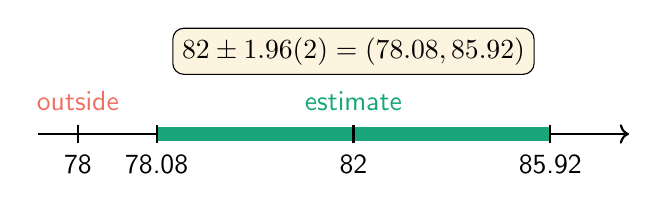
\begin{tikzpicture}[x=1cm,y=1cm]
\draw[->,thick] (-.5,0)--(7,0);
\draw[NovaGrowth,line width=5pt] (1,0)--(6,0);
\foreach \x/\lab in {0/78,1/78.08,3.5/82,6/85.92}{\draw[thick] (\x,-.12)--(\x,.12);\node[below] at (\x,-.15) {\lab};}
\node[NovaCoral,above] at (0,.18) {outside};\node[NovaGrowth,above] at (3.5,.18) {estimate};
\node[draw,rounded corners,fill=NovaYellow!20] at (3.5,1.05) {$82\pm1.96(2)=(78.08,85.92)$};
\end{tikzpicture}\end{center}
\end{column}
\end{columns}

\end{frame}

\begin{frame}{Big Idea}
\begin{columns}[T]
\begin{column}{0.53\textwidth}
\begin{alertblock}{Key idea}
\small Random samples vary. The distribution of their sample means has center mu and standard error sigma divided by the square root of n.
\end{alertblock}

\begin{block}{Mathematical relationship}
\centering\Large $\bar{x}\pm1.96\frac{\sigma}{\sqrt{n}}$\\[0.12cm]
\small A 95\% confidence interval for a mean with known population standard deviation.\ Same units as the measured variable
\end{block}

\begin{itemize}
\small
\item Distinguish a sample distribution from a sampling distribution.
\item Interpret standard error as sample-to-sample variability.
\item Compute and interpret a z-score and confidence interval.
\end{itemize}
\end{column}
\begin{column}{0.43\textwidth}
\begin{center}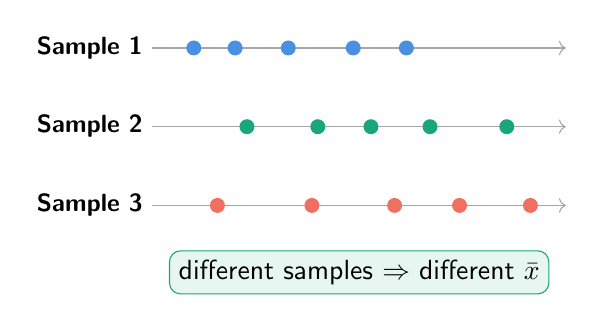
\begin{tikzpicture}[x=.75cm,y=1cm]
\foreach \y in {0,1,2}{\draw[->,gray!70] (-3.5,\y)--(3.5,\y);\node[left,font=\small\bfseries] at (-3.5,\y) {Sample \pgfmathparse{int(3-\y)}\pgfmathresult};}
\foreach \x in {-2.8,-2.1,-1.2,-.1,.8}{\fill[NovaSky] (\x,2) circle (2.7pt);}
\foreach \x in {-1.9,-.7,.2,1.2,2.5}{\fill[NovaGrowth] (\x,1) circle (2.7pt);}
\foreach \x in {-2.4,-.8,.6,1.7,2.9}{\fill[NovaCoral] (\x,0) circle (2.7pt);}
\node[draw=NovaGrowth,rounded corners,fill=NovaGrowth!10] at (0,-.85) {different samples $\Rightarrow$ different $\bar{x}$};
\end{tikzpicture}\end{center}
\end{column}
\end{columns}

\end{frame}

\begin{frame}{Key Words To Know}
\begin{columns}[T]
\begin{column}{0.53\textwidth}
\begin{alertblock}{Key idea}
\small These words unlock the lesson.
\end{alertblock}

\begin{block}{Mathematical relationship}
\centering\Large $\operatorname{SE}(\bar{x})=\frac{\sigma}{\sqrt{n}}$\\[0.12cm]
\small Standard error of the sample mean when population standard deviation is known.\ Same units as the measured variable
\end{block}

\begin{itemize}
\small
\item population
\item random sample
\item parameter
\end{itemize}
\end{column}
\begin{column}{0.43\textwidth}
\begin{center}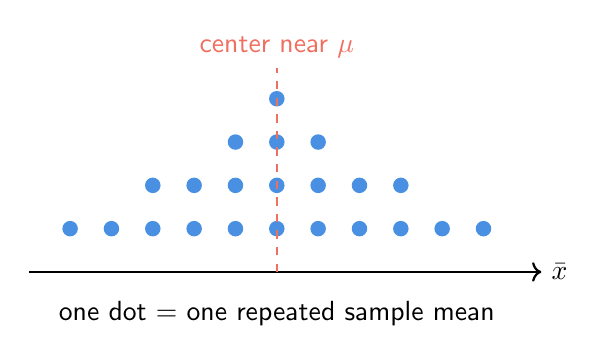
\begin{tikzpicture}[x=1.05cm,y=.55cm]
\draw[->,thick] (-3,0)--(3.2,0) node[right] {$\bar{x}$};
\foreach \x/\y in {-2.5/1,-2/1,-1.5/1,-1.5/2,-1/1,-1/2,-.5/1,-.5/2,-.5/3,0/1,0/2,0/3,0/4,.5/1,.5/2,.5/3,1/1,1/2,1.5/1,1.5/2,2/1,2.5/1}{\fill[NovaSky] (\x,\y) circle (2.8pt);}
\draw[dashed,NovaCoral,thick] (0,0)--(0,4.7) node[above] {center near $\mu$};
\node[below] at (0,-.45) {one dot = one repeated sample mean};
\end{tikzpicture}\end{center}
\end{column}
\end{columns}

\end{frame}

\begin{frame}{Before We Start}
\begin{columns}[T]
\begin{column}{0.53\textwidth}
\begin{alertblock}{Key idea}
\small Check the foundations first.
\end{alertblock}

\begin{block}{Mathematical relationship}
\centering\Large $\bar{x}\pm1.96\frac{\sigma}{\sqrt{n}}$\\[0.12cm]
\small A 95\% confidence interval for a mean with known population standard deviation.\ Same units as the measured variable
\end{block}

\begin{itemize}
\small
\item Find a mean.
\item Evaluate a square root.
\item Read an interval on a number line.
\end{itemize}
\end{column}
\begin{column}{0.43\textwidth}
\begin{center}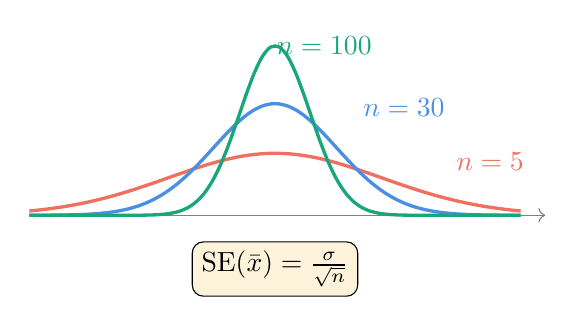
\begin{tikzpicture}[x=.78cm,y=1.05cm]
\draw[->,gray] (-4,0)--(4.4,0);
\draw[very thick,NovaCoral,domain=-4:4,samples=60,smooth] plot (\x,{.75*exp(-(\x)^2/6)});
\draw[very thick,NovaSky,domain=-4:4,samples=60,smooth] plot (\x,{1.35*exp(-(\x)^2/2)});
\draw[very thick,NovaGrowth,domain=-4:4,samples=60,smooth] plot (\x,{2.05*exp(-(\x)^2/.65)});
\node[NovaCoral] at (3.5,.65) {$n=5$};\node[NovaSky] at (2.1,1.3) {$n=30$};\node[NovaGrowth] at (.8,2.05) {$n=100$};
\node[draw,rounded corners,fill=NovaYellow!22] at (0,-.65) {$\operatorname{SE}(\bar{x})=\frac{\sigma}{\sqrt n}$};
\end{tikzpicture}\end{center}
\end{column}
\end{columns}

\end{frame}

\begin{frame}{Warm-up}
\begin{columns}[T]
\begin{column}{0.45\textwidth}
\begin{block}{Question}
\small Two random samples from the same population have different means. Is either sample necessarily wrong?
\end{block}
\end{column}
\begin{column}{0.51\textwidth}
\begin{center}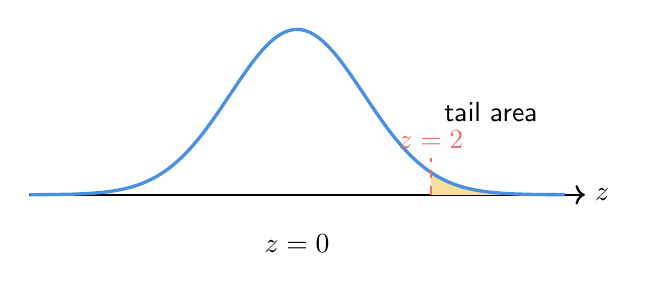
\begin{tikzpicture}[x=.85cm,y=2.1cm]
\draw[->,thick] (-4,0)--(4.3,0) node[right] {$z$};
\fill[NovaYellow!60,domain=2:4,samples=35] (2,0)--plot (\x,{exp(-(\x)^2/2)})--(4,0)--cycle;
\draw[very thick,NovaSky,domain=-4:4,samples=70,smooth] plot (\x,{exp(-(\x)^2/2)});
\draw[dashed,NovaCoral,thick] (2,0)--(2,.22) node[above] {$z=2$};
\node at (2.9,.5) {tail area};\node[below] at (0,-.18) {$z=0$};
\end{tikzpicture}\end{center}
\end{column}
\end{columns}

\end{frame}

\begin{frame}{Key Idea 1}
\begin{columns}[T]
\begin{column}{0.53\textwidth}
\begin{alertblock}{Key idea}
\small Understand the idea before memorizing details.
\end{alertblock}

\small Random samples vary. The distribution of their sample means has center mu and standard error sigma divided by the square root of n.

\begin{block}{Mathematical relationship}
\centering\Large $\operatorname{SE}(\bar{x})=\frac{\sigma}{\sqrt{n}}$\\[0.12cm]
\small Standard error of the sample mean when population standard deviation is known.\ Same units as the measured variable
\end{block}
\end{column}
\begin{column}{0.43\textwidth}
\begin{center}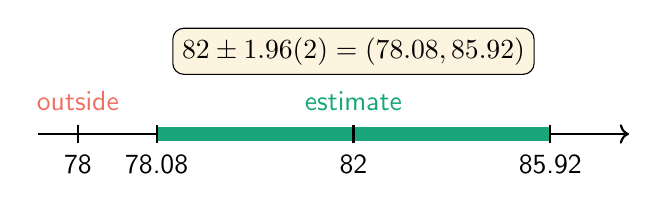
\begin{tikzpicture}[x=1cm,y=1cm]
\draw[->,thick] (-.5,0)--(7,0);
\draw[NovaGrowth,line width=5pt] (1,0)--(6,0);
\foreach \x/\lab in {0/78,1/78.08,3.5/82,6/85.92}{\draw[thick] (\x,-.12)--(\x,.12);\node[below] at (\x,-.15) {\lab};}
\node[NovaCoral,above] at (0,.18) {outside};\node[NovaGrowth,above] at (3.5,.18) {estimate};
\node[draw,rounded corners,fill=NovaYellow!20] at (3.5,1.05) {$82\pm1.96(2)=(78.08,85.92)$};
\end{tikzpicture}\end{center}
\end{column}
\end{columns}

\end{frame}

\begin{frame}{Population And Random Samples}
\begin{columns}[T]
\begin{column}{0.45\textwidth}
\begin{alertblock}{Key idea}
\small A population has fixed parameters. A random sample produces statistics that vary from sample to sample.
\end{alertblock}

\begin{itemize}
\small
\item Population: the full process or group.
\item Sample: observations selected by a random mechanism.
\end{itemize}
\end{column}
\begin{column}{0.51\textwidth}
\begin{center}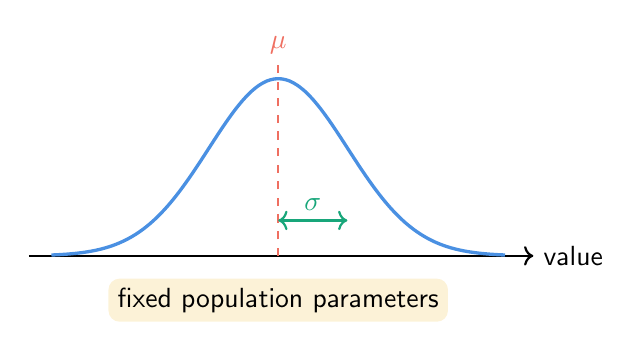
\begin{tikzpicture}[x=.72cm,y=2.25cm]
\draw[->,thick] (-4.4,0)--(4.5,0) node[right]{value};
\draw[very thick,NovaSky,domain=-4:4,samples=60,smooth] plot (\x,{exp(-(\x)^2/3)});
\draw[dashed,NovaCoral,thick] (0,0)--(0,1.08) node[above] {$\mu$};
\draw[<->,NovaGrowth,thick] (0,.2)--(1.22,.2) node[midway,above] {$\sigma$};
\node[fill=NovaYellow!25,rounded corners] at (0,-.25) {fixed population parameters};
\end{tikzpicture}\end{center}
\end{column}
\end{columns}

\end{frame}

\begin{frame}{Why Sample Means Vary}
\begin{columns}[T]
\begin{column}{0.45\textwidth}
\begin{alertblock}{Key idea}
\small Different random samples usually contain different observations, so their sample means are not identical.
\end{alertblock}
\end{column}
\begin{column}{0.51\textwidth}
\begin{center}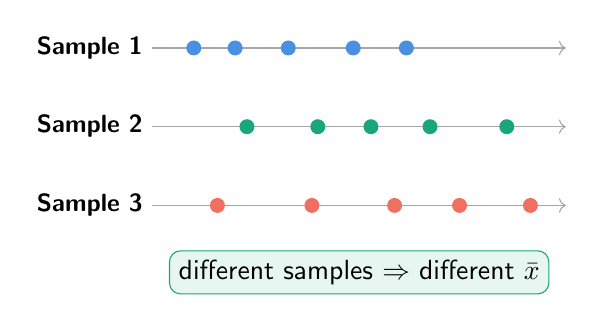
\begin{tikzpicture}[x=.75cm,y=1cm]
\foreach \y in {0,1,2}{\draw[->,gray!70] (-3.5,\y)--(3.5,\y);\node[left,font=\small\bfseries] at (-3.5,\y) {Sample \pgfmathparse{int(3-\y)}\pgfmathresult};}
\foreach \x in {-2.8,-2.1,-1.2,-.1,.8}{\fill[NovaSky] (\x,2) circle (2.7pt);}
\foreach \x in {-1.9,-.7,.2,1.2,2.5}{\fill[NovaGrowth] (\x,1) circle (2.7pt);}
\foreach \x in {-2.4,-.8,.6,1.7,2.9}{\fill[NovaCoral] (\x,0) circle (2.7pt);}
\node[draw=NovaGrowth,rounded corners,fill=NovaGrowth!10] at (0,-.85) {different samples $\Rightarrow$ different $\bar{x}$};
\end{tikzpicture}\end{center}
\end{column}
\end{columns}

\end{frame}

\begin{frame}{Build A Sampling Distribution}
\begin{columns}[T]
\begin{column}{0.53\textwidth}
\begin{alertblock}{Key idea}
\small Collecting one sample mean from each repeated sample creates the sampling distribution of the mean.
\end{alertblock}

\begin{block}{Mathematical relationship}
\centering\Large $\operatorname{SE}(\bar{x})=\frac{\sigma}{\sqrt{n}}$\\[0.12cm]
\small Standard error of the sample mean when population standard deviation is known.\ Same units as the measured variable
\end{block}

\begin{itemize}
\small
\item One dot represents one sample mean.
\item The center is near the population mean.
\end{itemize}
\end{column}
\begin{column}{0.43\textwidth}
\begin{center}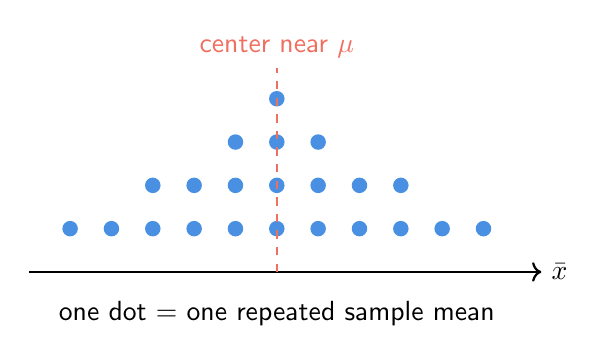
\begin{tikzpicture}[x=1.05cm,y=.55cm]
\draw[->,thick] (-3,0)--(3.2,0) node[right] {$\bar{x}$};
\foreach \x/\y in {-2.5/1,-2/1,-1.5/1,-1.5/2,-1/1,-1/2,-.5/1,-.5/2,-.5/3,0/1,0/2,0/3,0/4,.5/1,.5/2,.5/3,1/1,1/2,1.5/1,1.5/2,2/1,2.5/1}{\fill[NovaSky] (\x,\y) circle (2.8pt);}
\draw[dashed,NovaCoral,thick] (0,0)--(0,4.7) node[above] {center near $\mu$};
\node[below] at (0,-.45) {one dot = one repeated sample mean};
\end{tikzpicture}\end{center}
\end{column}
\end{columns}

\end{frame}

\begin{frame}{Sample Size Changes Precision}
\begin{columns}[T]
\begin{column}{0.53\textwidth}
\begin{alertblock}{Key idea}
\small For fixed population spread, larger samples produce a narrower sampling distribution.
\end{alertblock}

\begin{block}{Mathematical relationship}
\centering\Large $\widehat{\operatorname{SE}}(\bar{x})=\frac{s}{\sqrt{n}}$\\[0.12cm]
\small Estimated standard error of the sample mean.
\end{block}

\begin{itemize}
\small
\item Standard error is the standard deviation of the sampling distribution.
\item Quadrupling n halves the standard error.
\end{itemize}
\end{column}
\begin{column}{0.43\textwidth}
\begin{center}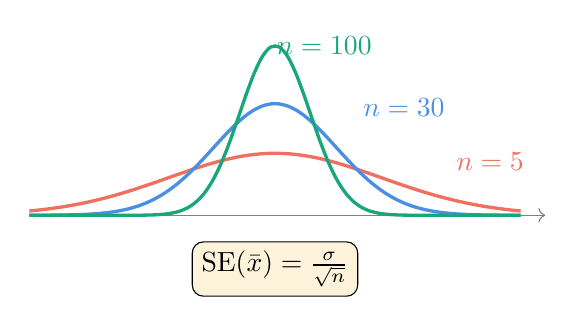
\begin{tikzpicture}[x=.78cm,y=1.05cm]
\draw[->,gray] (-4,0)--(4.4,0);
\draw[very thick,NovaCoral,domain=-4:4,samples=60,smooth] plot (\x,{.75*exp(-(\x)^2/6)});
\draw[very thick,NovaSky,domain=-4:4,samples=60,smooth] plot (\x,{1.35*exp(-(\x)^2/2)});
\draw[very thick,NovaGrowth,domain=-4:4,samples=60,smooth] plot (\x,{2.05*exp(-(\x)^2/.65)});
\node[NovaCoral] at (3.5,.65) {$n=5$};\node[NovaSky] at (2.1,1.3) {$n=30$};\node[NovaGrowth] at (.8,2.05) {$n=100$};
\node[draw,rounded corners,fill=NovaYellow!22] at (0,-.65) {$\operatorname{SE}(\bar{x})=\frac{\sigma}{\sqrt n}$};
\end{tikzpicture}\end{center}
\end{column}
\end{columns}

\end{frame}

\begin{frame}{Measure Distance With z}
\begin{columns}[T]
\begin{column}{0.53\textwidth}
\begin{alertblock}{Key idea}
\small A z-score is a signed distance measured in standard errors. It is not itself a probability.
\end{alertblock}

\begin{block}{Mathematical relationship}
\centering\Large $z=\frac{\bar{x}-\mu}{\sigma/\sqrt{n}}$\\[0.12cm]
\small One-sample z statistic for a sample mean.
\end{block}

\begin{itemize}
\small
\item Positive z is above the model mean.
\item Tail area converts location into probability.
\end{itemize}
\end{column}
\begin{column}{0.43\textwidth}
\begin{center}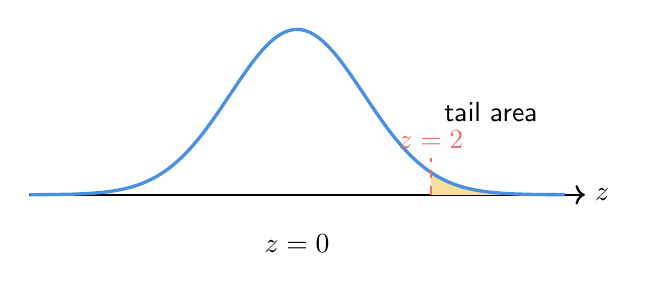
\begin{tikzpicture}[x=.85cm,y=2.1cm]
\draw[->,thick] (-4,0)--(4.3,0) node[right] {$z$};
\fill[NovaYellow!60,domain=2:4,samples=35] (2,0)--plot (\x,{exp(-(\x)^2/2)})--(4,0)--cycle;
\draw[very thick,NovaSky,domain=-4:4,samples=70,smooth] plot (\x,{exp(-(\x)^2/2)});
\draw[dashed,NovaCoral,thick] (2,0)--(2,.22) node[above] {$z=2$};
\node at (2.9,.5) {tail area};\node[below] at (0,-.18) {$z=0$};
\end{tikzpicture}\end{center}
\end{column}
\end{columns}

\end{frame}

\begin{frame}{Complete z And Interval Example}
\begin{columns}[T]
\begin{column}{0.53\textwidth}
\begin{alertblock}{Key idea}
\small Given \textbackslash\{\}bar\{x\}=82, \textbackslash\{\}mu=78, \textbackslash\{\}sigma=10, and n=25, first compute SE=2 and then z=2.
\end{alertblock}

\begin{block}{Mathematical relationship}
\centering\Large $\bar{x}\pm1.96\frac{\sigma}{\sqrt{n}}$\\[0.12cm]
\small A 95\% confidence interval for a mean with known population standard deviation.\ Same units as the measured variable
\end{block}

\begin{enumerate}
\small
\item Given: \textbackslash\{\}bar\{x\}=82, \textbackslash\{\}mu=78, \textbackslash\{\}sigma=10, n=25.
\item SE=10/\textbackslash\{\}sqrt\{25\}=2.
\item z=(82-78)/2=2.
\end{enumerate}
\end{column}
\begin{column}{0.43\textwidth}
\begin{center}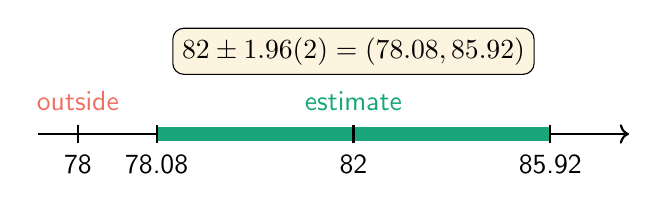
\begin{tikzpicture}[x=1cm,y=1cm]
\draw[->,thick] (-.5,0)--(7,0);
\draw[NovaGrowth,line width=5pt] (1,0)--(6,0);
\foreach \x/\lab in {0/78,1/78.08,3.5/82,6/85.92}{\draw[thick] (\x,-.12)--(\x,.12);\node[below] at (\x,-.15) {\lab};}
\node[NovaCoral,above] at (0,.18) {outside};\node[NovaGrowth,above] at (3.5,.18) {estimate};
\node[draw,rounded corners,fill=NovaYellow!20] at (3.5,1.05) {$82\pm1.96(2)=(78.08,85.92)$};
\end{tikzpicture}\end{center}
\end{column}
\end{columns}

\end{frame}

\begin{frame}{Choose z Or t}
\begin{columns}[T]
\begin{column}{0.53\textwidth}
\begin{alertblock}{Key idea}
\small Known population standard deviation supports a z-procedure. When it is unknown, estimate with s and normally use t with n-1 degrees of freedom.
\end{alertblock}

\begin{block}{Mathematical relationship}
\centering\Large $z=\frac{\bar{x}-\mu}{\sigma/\sqrt{n}}$\\[0.12cm]
\small One-sample z statistic for a sample mean.
\end{block}

\begin{itemize}
\small
\item Known \textbackslash\{\}sigma: SE=\textbackslash\{\}sigma/\textbackslash\{\}sqrt\{n\}.
\item Unknown \textbackslash\{\}sigma: estimated SE=s/\textbackslash\{\}sqrt\{n\} and use t.
\end{itemize}
\end{column}
\begin{column}{0.43\textwidth}
\begin{center}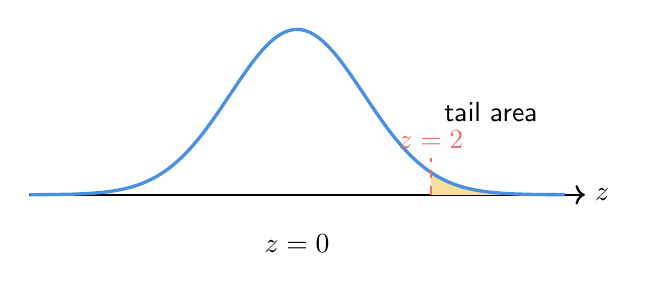
\begin{tikzpicture}[x=.85cm,y=2.1cm]
\draw[->,thick] (-4,0)--(4.3,0) node[right] {$z$};
\fill[NovaYellow!60,domain=2:4,samples=35] (2,0)--plot (\x,{exp(-(\x)^2/2)})--(4,0)--cycle;
\draw[very thick,NovaSky,domain=-4:4,samples=70,smooth] plot (\x,{exp(-(\x)^2/2)});
\draw[dashed,NovaCoral,thick] (2,0)--(2,.22) node[above] {$z=2$};
\node at (2.9,.5) {tail area};\node[below] at (0,-.18) {$z=0$};
\end{tikzpicture}\end{center}
\end{column}
\end{columns}

\end{frame}

\begin{frame}{Example: Given x bar 82}
\begin{columns}[T]
\begin{column}{0.53\textwidth}
\small Given x bar = 82, mu = 78, sigma = 10, and n = 25. Standard error is 2, z is 2, and the 95\% confidence interval is (78.08, 85.92). Therefore 78 is slightly outside the interval.

\begin{block}{Mathematical relationship}
\centering\Large $\bar{x}\pm1.96\frac{\sigma}{\sqrt{n}}$\\[0.12cm]
\small A 95\% confidence interval for a mean with known population standard deviation.\ Same units as the measured variable
\end{block}
\end{column}
\begin{column}{0.43\textwidth}
\begin{center}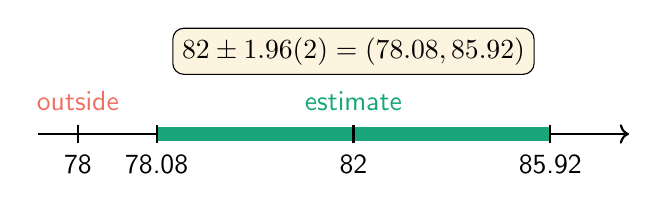
\begin{tikzpicture}[x=1cm,y=1cm]
\draw[->,thick] (-.5,0)--(7,0);
\draw[NovaGrowth,line width=5pt] (1,0)--(6,0);
\foreach \x/\lab in {0/78,1/78.08,3.5/82,6/85.92}{\draw[thick] (\x,-.12)--(\x,.12);\node[below] at (\x,-.15) {\lab};}
\node[NovaCoral,above] at (0,.18) {outside};\node[NovaGrowth,above] at (3.5,.18) {estimate};
\node[draw,rounded corners,fill=NovaYellow!20] at (3.5,1.05) {$82\pm1.96(2)=(78.08,85.92)$};
\end{tikzpicture}\end{center}
\end{column}
\end{columns}

\end{frame}

\begin{frame}{Practice 1}
\begin{columns}[T]
\begin{column}{0.53\textwidth}
\begin{block}{Question}
\small Known sigma is 12 and n is 36. Find the standard error without revealing the answer first.
\end{block}

\begin{block}{Mathematical relationship}
\centering\Large $\operatorname{SE}(\bar{x})=\frac{\sigma}{\sqrt{n}}$\\[0.12cm]
\small Standard error of the sample mean when population standard deviation is known.\ Same units as the measured variable
\end{block}
\end{column}
\begin{column}{0.43\textwidth}
\begin{center}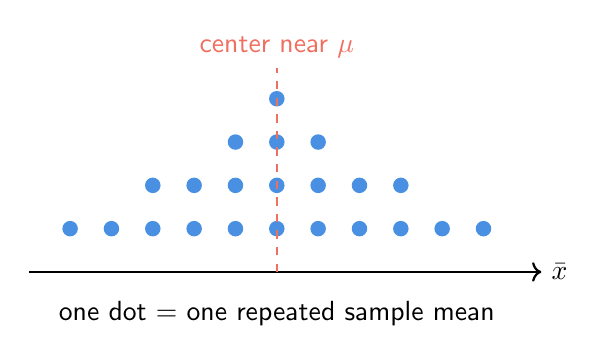
\begin{tikzpicture}[x=1.05cm,y=.55cm]
\draw[->,thick] (-3,0)--(3.2,0) node[right] {$\bar{x}$};
\foreach \x/\y in {-2.5/1,-2/1,-1.5/1,-1.5/2,-1/1,-1/2,-.5/1,-.5/2,-.5/3,0/1,0/2,0/3,0/4,.5/1,.5/2,.5/3,1/1,1/2,1.5/1,1.5/2,2/1,2.5/1}{\fill[NovaSky] (\x,\y) circle (2.8pt);}
\draw[dashed,NovaCoral,thick] (0,0)--(0,4.7) node[above] {center near $\mu$};
\node[below] at (0,-.45) {one dot = one repeated sample mean};
\end{tikzpicture}\end{center}
\end{column}
\end{columns}

\end{frame}

\begin{frame}{Practice 2}
\begin{columns}[T]
\begin{column}{0.53\textwidth}
\begin{block}{Question}
\small A sample mean is 50, mu is 45, sigma is 8, and n is 16. Find and interpret z.
\end{block}

\begin{block}{Mathematical relationship}
\centering\Large $z=\frac{\bar{x}-\mu}{\sigma/\sqrt{n}}$\\[0.12cm]
\small One-sample z statistic for a sample mean.
\end{block}
\end{column}
\begin{column}{0.43\textwidth}
\begin{center}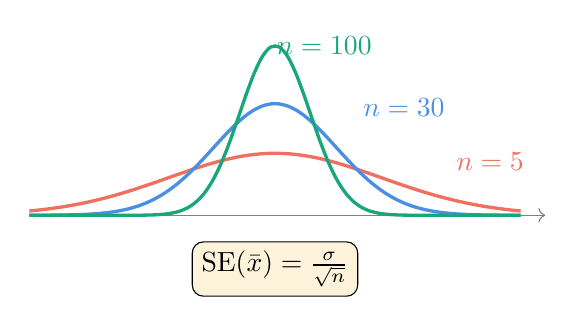
\begin{tikzpicture}[x=.78cm,y=1.05cm]
\draw[->,gray] (-4,0)--(4.4,0);
\draw[very thick,NovaCoral,domain=-4:4,samples=60,smooth] plot (\x,{.75*exp(-(\x)^2/6)});
\draw[very thick,NovaSky,domain=-4:4,samples=60,smooth] plot (\x,{1.35*exp(-(\x)^2/2)});
\draw[very thick,NovaGrowth,domain=-4:4,samples=60,smooth] plot (\x,{2.05*exp(-(\x)^2/.65)});
\node[NovaCoral] at (3.5,.65) {$n=5$};\node[NovaSky] at (2.1,1.3) {$n=30$};\node[NovaGrowth] at (.8,2.05) {$n=100$};
\node[draw,rounded corners,fill=NovaYellow!22] at (0,-.65) {$\operatorname{SE}(\bar{x})=\frac{\sigma}{\sqrt n}$};
\end{tikzpicture}\end{center}
\end{column}
\end{columns}

\end{frame}

\begin{frame}{Common Mistake To Avoid}
\begin{columns}[T]
\begin{column}{0.45\textwidth}
\begin{alertblock}{Key idea}
\small Mistakes become easier to catch when you know what to look for.
\end{alertblock}

\begin{itemize}
\small
\item Do not multiply only one quantity in a ratio.
\item Equivalent ratios need the same scale factor on both quantities.
\end{itemize}
\end{column}
\begin{column}{0.51\textwidth}
\begin{center}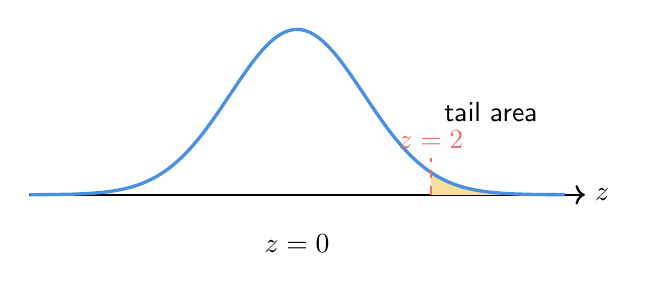
\begin{tikzpicture}[x=.85cm,y=2.1cm]
\draw[->,thick] (-4,0)--(4.3,0) node[right] {$z$};
\fill[NovaYellow!60,domain=2:4,samples=35] (2,0)--plot (\x,{exp(-(\x)^2/2)})--(4,0)--cycle;
\draw[very thick,NovaSky,domain=-4:4,samples=70,smooth] plot (\x,{exp(-(\x)^2/2)});
\draw[dashed,NovaCoral,thick] (2,0)--(2,.22) node[above] {$z=2$};
\node at (2.9,.5) {tail area};\node[below] at (0,-.18) {$z=0$};
\end{tikzpicture}\end{center}
\end{column}
\end{columns}

\end{frame}

\begin{frame}{Show What You Know}
\begin{columns}[T]
\begin{column}{0.53\textwidth}
\begin{block}{Question}
\small What does one dot in a sampling distribution represent?
\end{block}

\begin{block}{Mathematical relationship}
\centering\Large $\operatorname{SE}(\bar{x})=\frac{\sigma}{\sqrt{n}}$\\[0.12cm]
\small Standard error of the sample mean when population standard deviation is known.\ Same units as the measured variable
\end{block}
\end{column}
\begin{column}{0.43\textwidth}
\begin{center}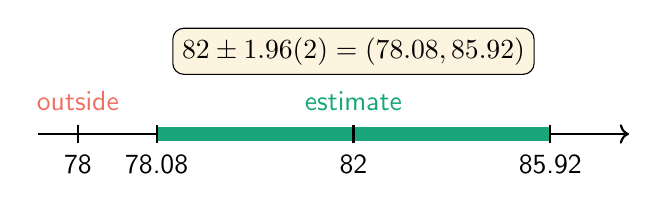
\begin{tikzpicture}[x=1cm,y=1cm]
\draw[->,thick] (-.5,0)--(7,0);
\draw[NovaGrowth,line width=5pt] (1,0)--(6,0);
\foreach \x/\lab in {0/78,1/78.08,3.5/82,6/85.92}{\draw[thick] (\x,-.12)--(\x,.12);\node[below] at (\x,-.15) {\lab};}
\node[NovaCoral,above] at (0,.18) {outside};\node[NovaGrowth,above] at (3.5,.18) {estimate};
\node[draw,rounded corners,fill=NovaYellow!20] at (3.5,1.05) {$82\pm1.96(2)=(78.08,85.92)$};
\end{tikzpicture}\end{center}
\end{column}
\end{columns}

\end{frame}

\begin{frame}{Check 2}
\begin{columns}[T]
\begin{column}{0.53\textwidth}
\begin{block}{Question}
\small Why does quadrupling n halve standard error?
\end{block}

\begin{block}{Mathematical relationship}
\centering\Large $\operatorname{SE}(\bar{x})=\frac{\sigma}{\sqrt{n}}$\\[0.12cm]
\small Standard error of the sample mean when population standard deviation is known.\ Same units as the measured variable
\end{block}
\end{column}
\begin{column}{0.43\textwidth}
\begin{center}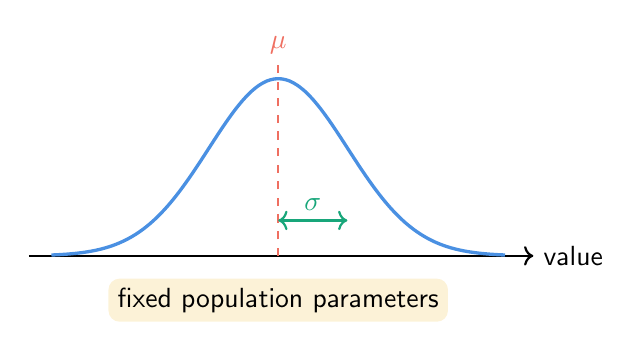
\begin{tikzpicture}[x=.72cm,y=2.25cm]
\draw[->,thick] (-4.4,0)--(4.5,0) node[right]{value};
\draw[very thick,NovaSky,domain=-4:4,samples=60,smooth] plot (\x,{exp(-(\x)^2/3)});
\draw[dashed,NovaCoral,thick] (0,0)--(0,1.08) node[above] {$\mu$};
\draw[<->,NovaGrowth,thick] (0,.2)--(1.22,.2) node[midway,above] {$\sigma$};
\node[fill=NovaYellow!25,rounded corners] at (0,-.25) {fixed population parameters};
\end{tikzpicture}\end{center}
\end{column}
\end{columns}

\end{frame}

\begin{frame}{Check 3}
\begin{columns}[T]
\begin{column}{0.53\textwidth}
\begin{block}{Question}
\small When sigma is unknown, why is a t-procedure normally used?
\end{block}

\begin{block}{Mathematical relationship}
\centering\Large $\widehat{\operatorname{SE}}(\bar{x})=\frac{s}{\sqrt{n}}$\\[0.12cm]
\small Estimated standard error of the sample mean.
\end{block}
\end{column}
\begin{column}{0.43\textwidth}
\begin{center}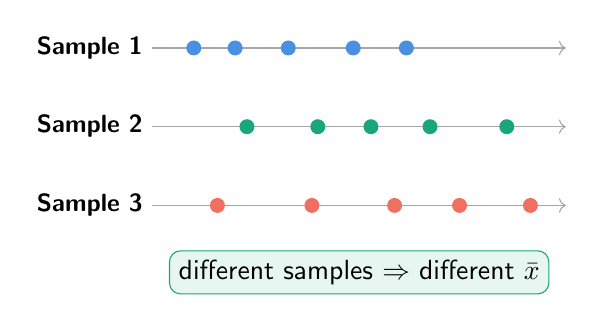
\begin{tikzpicture}[x=.75cm,y=1cm]
\foreach \y in {0,1,2}{\draw[->,gray!70] (-3.5,\y)--(3.5,\y);\node[left,font=\small\bfseries] at (-3.5,\y) {Sample \pgfmathparse{int(3-\y)}\pgfmathresult};}
\foreach \x in {-2.8,-2.1,-1.2,-.1,.8}{\fill[NovaSky] (\x,2) circle (2.7pt);}
\foreach \x in {-1.9,-.7,.2,1.2,2.5}{\fill[NovaGrowth] (\x,1) circle (2.7pt);}
\foreach \x in {-2.4,-.8,.6,1.7,2.9}{\fill[NovaCoral] (\x,0) circle (2.7pt);}
\node[draw=NovaGrowth,rounded corners,fill=NovaGrowth!10] at (0,-.85) {different samples $\Rightarrow$ different $\bar{x}$};
\end{tikzpicture}\end{center}
\end{column}
\end{columns}

\end{frame}

\begin{frame}{Quick Review}
\begin{columns}[T]
\begin{column}{0.53\textwidth}
\begin{alertblock}{Key idea}
\small A strong finish means you can explain the idea in your own words.
\end{alertblock}

\begin{block}{Mathematical relationship}
\centering\Large $\bar{x}\pm1.96\frac{\sigma}{\sqrt{n}}$\\[0.12cm]
\small A 95\% confidence interval for a mean with known population standard deviation.\ Same units as the measured variable
\end{block}

\begin{itemize}
\small
\item Distinguish a sample distribution from a sampling distribution.
\item Interpret standard error as sample-to-sample variability.
\item Compute and interpret a z-score and confidence interval.
\end{itemize}
\end{column}
\begin{column}{0.43\textwidth}
\begin{center}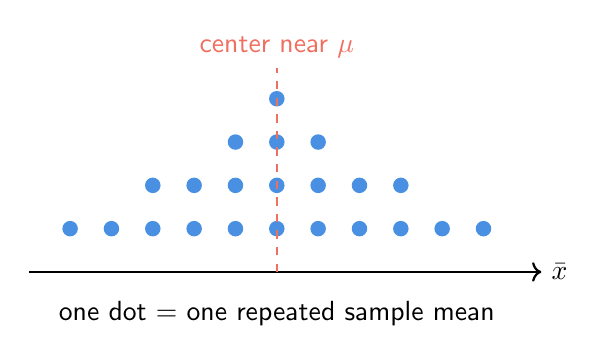
\begin{tikzpicture}[x=1.05cm,y=.55cm]
\draw[->,thick] (-3,0)--(3.2,0) node[right] {$\bar{x}$};
\foreach \x/\y in {-2.5/1,-2/1,-1.5/1,-1.5/2,-1/1,-1/2,-.5/1,-.5/2,-.5/3,0/1,0/2,0/3,0/4,.5/1,.5/2,.5/3,1/1,1/2,1.5/1,1.5/2,2/1,2.5/1}{\fill[NovaSky] (\x,\y) circle (2.8pt);}
\draw[dashed,NovaCoral,thick] (0,0)--(0,4.7) node[above] {center near $\mu$};
\node[below] at (0,-.45) {one dot = one repeated sample mean};
\end{tikzpicture}\end{center}
\end{column}
\end{columns}

\end{frame}

\begin{frame}{Recommended Next Session}
\begin{columns}[T]
\begin{column}{0.53\textwidth}
\begin{alertblock}{Key idea}
\small Use simulation to connect z-scores with one-sided and two-sided probabilities.
\end{alertblock}

\begin{block}{Question}
\small What should we practice next?
\end{block}

\begin{block}{Mathematical relationship}
\centering\Large $z=\frac{\bar{x}-\mu}{\sigma/\sqrt{n}}$\\[0.12cm]
\small One-sample z statistic for a sample mean.
\end{block}
\end{column}
\begin{column}{0.43\textwidth}
\begin{center}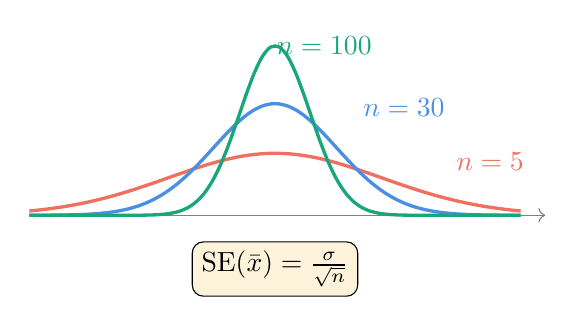
\begin{tikzpicture}[x=.78cm,y=1.05cm]
\draw[->,gray] (-4,0)--(4.4,0);
\draw[very thick,NovaCoral,domain=-4:4,samples=60,smooth] plot (\x,{.75*exp(-(\x)^2/6)});
\draw[very thick,NovaSky,domain=-4:4,samples=60,smooth] plot (\x,{1.35*exp(-(\x)^2/2)});
\draw[very thick,NovaGrowth,domain=-4:4,samples=60,smooth] plot (\x,{2.05*exp(-(\x)^2/.65)});
\node[NovaCoral] at (3.5,.65) {$n=5$};\node[NovaSky] at (2.1,1.3) {$n=30$};\node[NovaGrowth] at (.8,2.05) {$n=100$};
\node[draw,rounded corners,fill=NovaYellow!22] at (0,-.65) {$\operatorname{SE}(\bar{x})=\frac{\sigma}{\sqrt n}$};
\end{tikzpicture}\end{center}
\end{column}
\end{columns}

\end{frame}
\end{document}
